% Options for packages loaded elsewhere
\PassOptionsToPackage{unicode}{hyperref}
\PassOptionsToPackage{hyphens}{url}
%
\documentclass[
]{article}
\usepackage{lmodern}
\usepackage{amssymb,amsmath}
\usepackage{ifxetex,ifluatex}
\ifnum 0\ifxetex 1\fi\ifluatex 1\fi=0 % if pdftex
  \usepackage[T1]{fontenc}
  \usepackage[utf8]{inputenc}
  \usepackage{textcomp} % provide euro and other symbols
\else % if luatex or xetex
  \usepackage{unicode-math}
  \defaultfontfeatures{Scale=MatchLowercase}
  \defaultfontfeatures[\rmfamily]{Ligatures=TeX,Scale=1}
\fi
% Use upquote if available, for straight quotes in verbatim environments
\IfFileExists{upquote.sty}{\usepackage{upquote}}{}
\IfFileExists{microtype.sty}{% use microtype if available
  \usepackage[]{microtype}
  \UseMicrotypeSet[protrusion]{basicmath} % disable protrusion for tt fonts
}{}
\makeatletter
\@ifundefined{KOMAClassName}{% if non-KOMA class
  \IfFileExists{parskip.sty}{%
    \usepackage{parskip}
  }{% else
    \setlength{\parindent}{0pt}
    \setlength{\parskip}{6pt plus 2pt minus 1pt}}
}{% if KOMA class
  \KOMAoptions{parskip=half}}
\makeatother
\usepackage{xcolor}
\IfFileExists{xurl.sty}{\usepackage{xurl}}{} % add URL line breaks if available
\IfFileExists{bookmark.sty}{\usepackage{bookmark}}{\usepackage{hyperref}}
\hypersetup{
  pdftitle={CTT Locator User Manual},
  pdfauthor={support@celltracktech.com},
  hidelinks,
  pdfcreator={LaTeX via pandoc}}
\urlstyle{same} % disable monospaced font for URLs
\usepackage[margin=1in]{geometry}
\usepackage{graphicx,grffile}
\makeatletter
\def\maxwidth{\ifdim\Gin@nat@width>\linewidth\linewidth\else\Gin@nat@width\fi}
\def\maxheight{\ifdim\Gin@nat@height>\textheight\textheight\else\Gin@nat@height\fi}
\makeatother
% Scale images if necessary, so that they will not overflow the page
% margins by default, and it is still possible to overwrite the defaults
% using explicit options in \includegraphics[width, height, ...]{}
\setkeys{Gin}{width=\maxwidth,height=\maxheight,keepaspectratio}
% Set default figure placement to htbp
\makeatletter
\def\fps@figure{htbp}
\makeatother
\setlength{\emergencystretch}{3em} % prevent overfull lines
\providecommand{\tightlist}{%
  \setlength{\itemsep}{0pt}\setlength{\parskip}{0pt}}
\setcounter{secnumdepth}{-\maxdimen} % remove section numbering

\title{CTT Locator User Manual}
\author{\href{mailto:support@celltracktech.com}{\nolinkurl{support@celltracktech.com}}}
\date{3/12/2021}

\begin{document}
\maketitle

{
\setcounter{tocdepth}{2}
\tableofcontents
}
\hypertarget{the-ctt-locator}{%
\subsection{The CTT Locator}\label{the-ctt-locator}}

The CTT Locator is a portal device that can receive a variety of
wildlife tag signals. It is compatible with the entire radio tag line,
including ES200 devices.

\hypertarget{getting-started}{%
\section{Getting Started}\label{getting-started}}

\hypertarget{in-the-box}{%
\subsection{In the Box}\label{in-the-box}}

\begin{itemize}
\tightlist
\item
  Yagi Antenna
\item
  BNC to SMA coaxial adapter
\item
  SMA coaxial cable
\item
  CTT Locator with integrated Lithium Polymer battery and USB charger
  port
\end{itemize}

\hypertarget{powering-on-the-locator}{%
\section{Powering on the Locator}\label{powering-on-the-locator}}

\begin{enumerate}
\def\labelenumi{\arabic{enumi}.}
\tightlist
\item
  To power on the Locator, press the switch to on. A blue light will
  immediately shine, indicating the Locator has power. After a short
  bootup sequence, the Locator will create a hotspot for your phone to
  connect to. \textbf{Due to technical limitations, Android phones will
  need to turn off Cellular Data. This is not required on iPhone
  devices.} In addition to phones, the Locator can be used with laptops,
  tablets, and other modern devices.
\end{enumerate}

When the blue light flashes, the Locator is in its final stages of
booting. It will be ready in about 10 seconds after this indication.

\begin{enumerate}
\def\labelenumi{\arabic{enumi}.}
\setcounter{enumi}{1}
\item
  Connect to a WiFi network created by the Locator.
\item
  Enter this full url into the browser. Note that the \texttt{https://}
  is important:
\end{enumerate}

\begin{verbatim}
https://locator.click/
\end{verbatim}

In a few moments, a webpage will load and show the main locator screen.

\hypertarget{screen-overview}{%
\section{Screen Overview}\label{screen-overview}}

When you load the Locator screen, an interface will appear. You can
change the various modes of the locator by clicking on the icons at the
bottom.

First, we will go over the title bar:

The circle on the right will flash red when a tag is detected. A
rotating circle animation indicates that the locator is actively
connected to the phone. The far right icon indicates battery life, and
contains the voltage. Approximately 4.10 volts is a full battery, 3.7
volts is half full, and 3.4 volts is empty. This will also be indicated
by the battery slowly reducing, similar to your smart phone.

Next we will go over the icons at the bottom:

\begin{itemize}
\item
  The \texttt{Home} icon shows all detected tags in a list, which is the
  default view when you first connect to the device. For more details,
  see the Home View section.
\item
  The \texttt{Identify} icon helps you identify unknown tags or verify a
  tag's ID when it is in close range. For more details, see the Identify
  View section.
\item
  The \texttt{Favorites} icon is a place where you can see the tags you
  have specified as favorites. This is useful when a lot of other tags
  are nearby and you wish to focus on a specific tag. For more details,
  see the Favorites View section.
\item
  The \texttt{Search} icon is where you can search for tags within all
  of the tags recently detected during your session. For more details,
  see the Search View section.
\item
  The \texttt{Download} icon allows you to download all collected tag
  data as well as ES200 data. For more details, see the Download View
  section.
\item
  The \texttt{Settings} icon allows you to control various locator
  settings and options. For more details, see the Settings View section.
\end{itemize}

\hypertarget{home-view}{%
\section{Home View}\label{home-view}}

The \texttt{home} view shows all nearby tags. If a tag is first seen, it
will show up as red, to indicate a new tag has been detected. If the tag
is seen again, it will turn black. Each time the tag is detected, the
text will briefly flash yellow to indicate it has been updated.

\begin{figure}
\centering
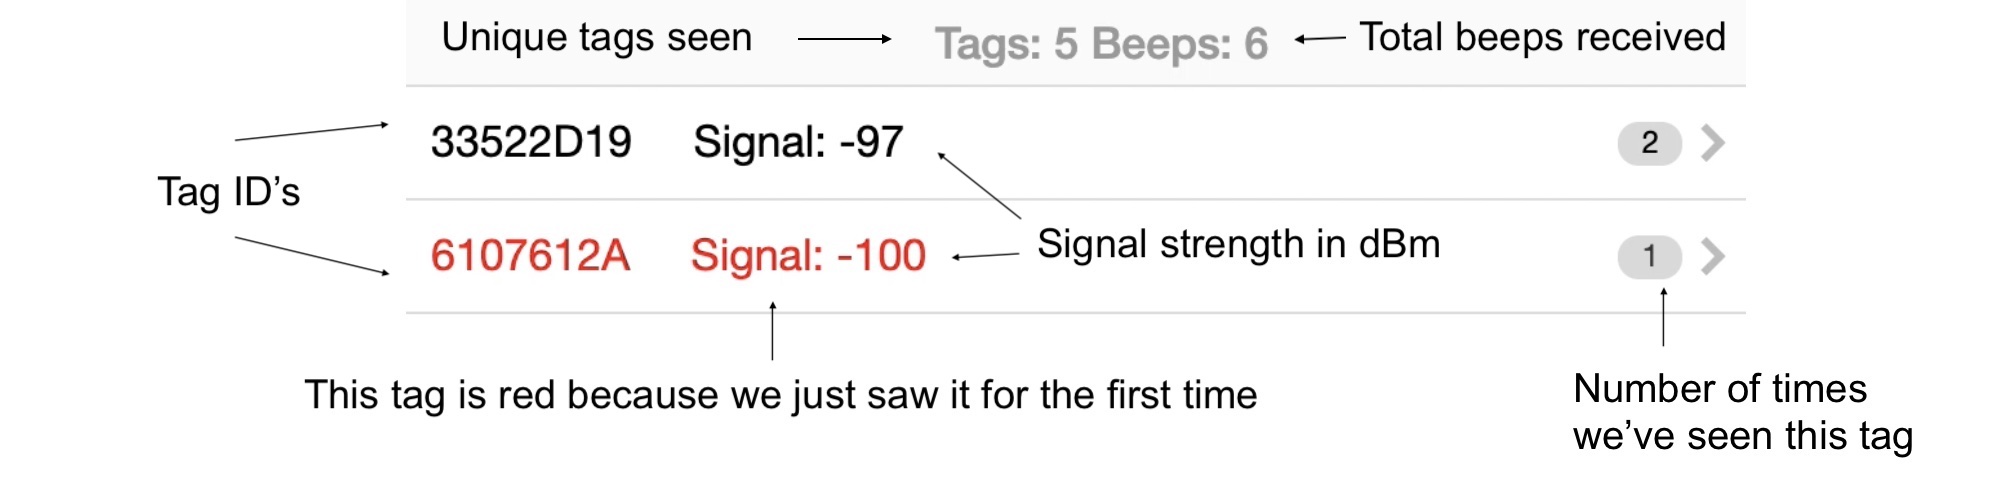
\includegraphics{https://user-images.githubusercontent.com/1101026/110704154-94803200-81c2-11eb-9a92-9746662533c3.jpg}
\caption{\emph{Locator main view}}
\end{figure}

\hypertarget{tag-view}{%
\section{Tag View}\label{tag-view}}

The \texttt{tag} view provides a signal strength indicator to help you
localize a tag. As the tag signal gets stronger, more bars appear. the
negative number under the signal bars is the signal strength in dBm, or
decibel milliwatts. The lower the number, the weaker the signal.

A large circle is at the top of the Tag View. This flashes when the tag
is received. Under this is the last time the tag was seen.

Touching or clicking the X in the top right corner closes tha tag view.

You can add a tag to your favorites list by tapping the ``Favorite''
button. Tapping this again removes the tag from your favorites.

\hypertarget{identify-view}{%
\section{Identify View}\label{identify-view}}

In the \texttt{Identify} view, tags will appear if they have signals
stronger than -30 dBm. This would be a tag in very close proximity to
the locator.

\hypertarget{favorite-view}{%
\section{Favorite View}\label{favorite-view}}

Any tags that are selected as favorites will enter the \texttt{Favorite}
view. You can click on any tag here to see the Tag View of any tag in
this list, just as you would in the main view.

\hypertarget{search-view}{%
\section{Search View}\label{search-view}}

The \texttt{Search} view lets you type in a tag ID, which is then
searched against tags detected during that session. Note that the
history of tags clears each time you open or reload the locator
interface. It will not search against any tag ever detected with the
locator.

\hypertarget{download-view}{%
\section{Download View}\label{download-view}}

The \texttt{Download} view is where you can download both ES200 and Tag
Data. Clicking on these will initiate a download to your device.

\hypertarget{settings-view}{%
\section{Settings View}\label{settings-view}}

\end{document}
